\chapter{Domain Driven Design}
\label{ch:ddd} %Label of the chapter lit rev. The key ``ch:lit_rev'' can be used with command \ref{ch:lit_rev} to refer this Chapter.

\section{Knowledge crunching session for the exploration of the problem space}
Per ottenere maggior chiarezza sul dominio è stato utilizzato il metodo Even Storming. 
La tecnica consiste nell'individuare degli eventi di dominio e riportarli al passato su un post-it arancione.
Una volta individuati gli eventi, sono stati scritti su post-it blu i comandi che l'utente svolge per creare l'evento.
In giallo è stato specificato l'attore, la persona che esegue il comando, mentre in verde la view, l'interfaccia software
 con la quale l'utente interagisce.
 Infine, con delle label si sono aggregati i post-it in unità di dominio.
 Si riporta di seguito lo screen della lavagna con i post-it e la relativa legenda.
 \begin{figure}[h!]
    \centering 
    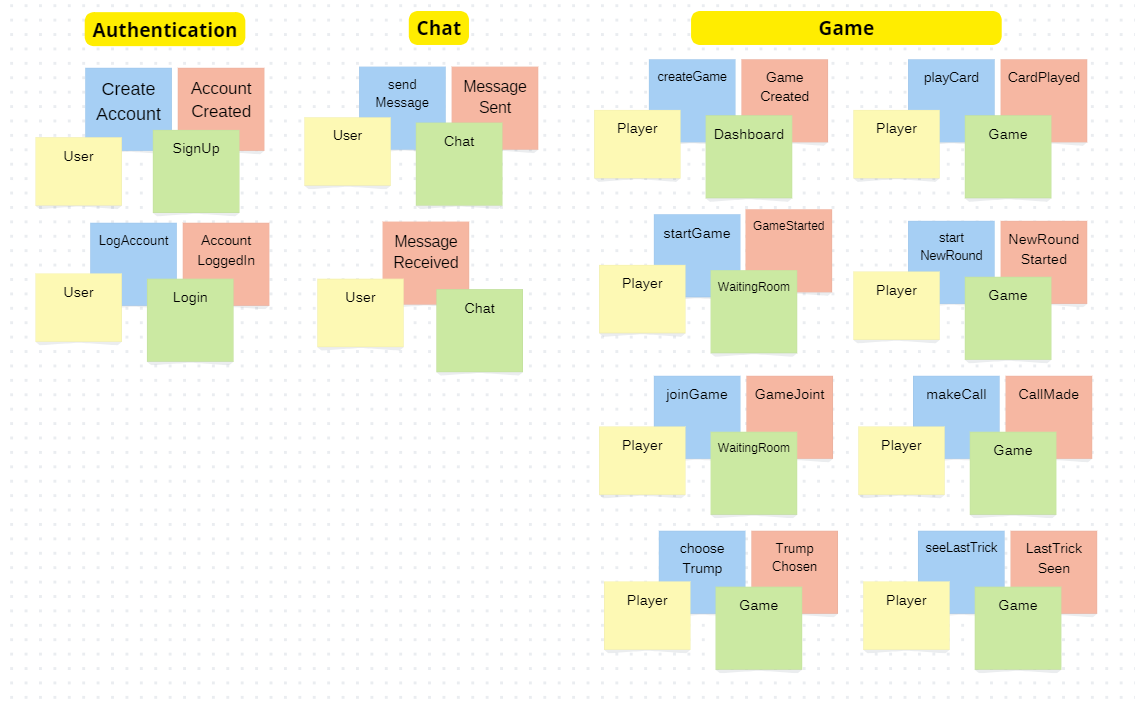
\includegraphics[scale=0.45]{report/img/EventStorming.png}
    \caption{Event Storming}
    \label{event_storming}
\end{figure}

\begin{figure}[h!]
    \centering 
    \includegraphics[scale=0.60]{report/img/Event_storming_legend.png}
    \caption{Event Storming Legend}
    \label{legend}
\end{figure}

\newpage



\section{Ubiquitos Language}
\begin{table}[!ht]
    \centering
    \begin{adjustbox}{max width=1.1\textwidth,center}
    \begin{tabular}{|l|p{10cm}|l|}
    \hline
        Nome & Descrizione & Sinonimi \\ \hline
        Mano & Distribuzione delle 40 carte ai 4 giocatori e la seguente serie di 10 prese & Round \\ \hline
        Mano & Carte dei giocatori non ancora giocate & Hand \\ \hline
        Presa & Quando ogni giocatore, a turno, gioca sul tavolo una carta. L’ultima presa della mano vale 1 punto. & Trick \\ \hline
        Partita & Insieme di più mani fino al raggiungimento del punteggio di 41 punti. & Game \\ \hline
        Partita corta & Insieme di più mani fino al raggiungimento del punteggio di 31 punti. & Short Game \\ \hline
        Tavolo & Raggruppamento di 4 giocatori, suddivisi in 2 coppie, i giocatori delle stessa squadra “siedono” in direzione opposta & Table \\ \hline
        Seme & Tipologia distintiva di carta, ne esistono 4: Denari, Coppe, Spade, Bastoni & Suit: Coins, Cups, Swords, Clubs~ \\ \hline
        Briscola & Seme con priorita’ piu’ alta. & Trump \\ \hline
        Maraffa & Se un giocatore possiede le tre carte di valore maggiore (asso, due e tre, dette assieme "Maraffa" o "Cricca")
        del seme di briscola, vince tre punti addizionali. In questo caso deve scendere con l'asso di quel seme. & Cricca, Marafon, Tresette con la Briscola \\ \hline
        Mazzo & 40 carte, di 4 semi diversi, 1,2,3,4,5,6,7, fante, cavallo e re. & Deck \\ \hline
        Taglio & Durante una mano in un seme viene giocato il seme di briscola, che avendo priorita’ maggiore
        permette di prendere nonostante il seme di gioco & Cut \\ \hline
        Busso & Invita il compagno, se possibile, a conquistare la presa e ad aprire il turno successivo con lo stesso seme & Knock \\ \hline
        Striscio corto & Quando si ha ancora in mano un basso numero di carte dello stesso seme con cui si è aperto il turno. & Short strip \\ \hline
        Striscio lungo & Quando si ha ancora in mano molte carte dello stesso seme con cui si è aperto il turno. & Long strip \\ \hline
        Volo & Quando non si hanno più carte del seme con cui si è aperto il turno. & Fly \\ \hline
        Figura & Fante, Cavallo, Re, con punteggio di 1/3 di punto. & Figure \\ \hline
        Asso & Carta con valore di 1 punto. & Ace \\ \hline
        Due e Tre & Carte con valore 1/3 di punto. & Two and Three \\ \hline
        Carta Liscia & Carte con numeri 4, 5, 6, 7. Sono prive di valore & Smooth paper \\ \hline
        Squadra & Coppie di giocatori seduti opposti & Team \\ \hline
        Giocatore & Persona che interagisce con l’applicativo & Player, User \\ \hline
        Chiamata fuori & Se un giocatore pensa che la sua squadra abbia raggiunto i 41 punti (o 31 punti nella variante "corta" della partita), la squadra può  dichiarare di avere già nel mazzo delle prese i punti per vincere e chiudere in anticipo l'ultima partita. In questo modo la mano termina immediatamente, senza che vengano giocate le restanti prese e la squadra che si è "chiamata fuori" impedisce all'altra squadra di conquistare ulteriori prese. Se una squadra si chiama fuori e, dopo aver contato i punti delle prese effettuate ed averli sommati ai punti ottenuti nelle mani già giocate, non raggiunge i punti per la vittoria (in gergo "sbaglia la chiamata") scatta automatico l'11 a 0 per la squadra avversaria & Call out \\ \hline
        Modalità di gioco & regole di gioco classiche o varianti che influenzano aspetti come il punteggio, condizioni di vittoria/perdita, ... Ne sono state implementate due: classica, 11 a 0.& Game mode \\ \hline
    \end{tabular}
    \end{adjustbox}
\end{table}
\newpage
\section{Bounded Context}
Analizzando il dominio di MaraffaOnline, sono stati identificati tre bounded context.
Nella figura si può osservare un primo bounded context, colorato di azzurro, che modella l'autenticazione dell'utente:
    \begin{itemize}
        \item \textbf{User:} persona che possiede l'account
        \item \textbf{Statistic:} dati dell'utente relativi al gioco come numero di vittorie, sconfitte, partite giocate e maraffe
        \item \textbf{Authentication:} accesso all'applicativo MaraffaOnline da parte dell'utente
    \end{itemize}
Il secondo bounded context, colorato di verde, modella la partita:
    \begin{itemize}
        \item \textbf{Game:} partita
        \item \textbf{Team:} squadra composta da numero di giocatori / 2
        \item \textbf{Score:} punteggio delle due squadre
        \item \textbf{Statistic:} dati relativi ai game giocati
        \item \textbf{Trick:} presa di quattro carte da parte di un giocatore
        \item \textbf{Round:} 10 prese
        \item \textbf{Card:} carta
        \item \textbf{Player:} giocatore
        \item \textbf{Deck:} mazzo
        \item \textbf{Hand:} carte che ha in mano un giocatore
    \end{itemize}
Infine l'ultimo, di colore arancione, modella la chat:
    \begin{itemize}
        \item \textbf{Chat:} chat di gioco
        \item \textbf{Message:} messaggio inviato nella chat
        \item \textbf{User:} persona che invia il messaggio
    \end{itemize}
È importante notare che il concetto di user/player è polisemico: vi sono tre rappresentazioni diverse per afferire allo stesso concetto.
\begin{figure}[h!]
    \centering 
    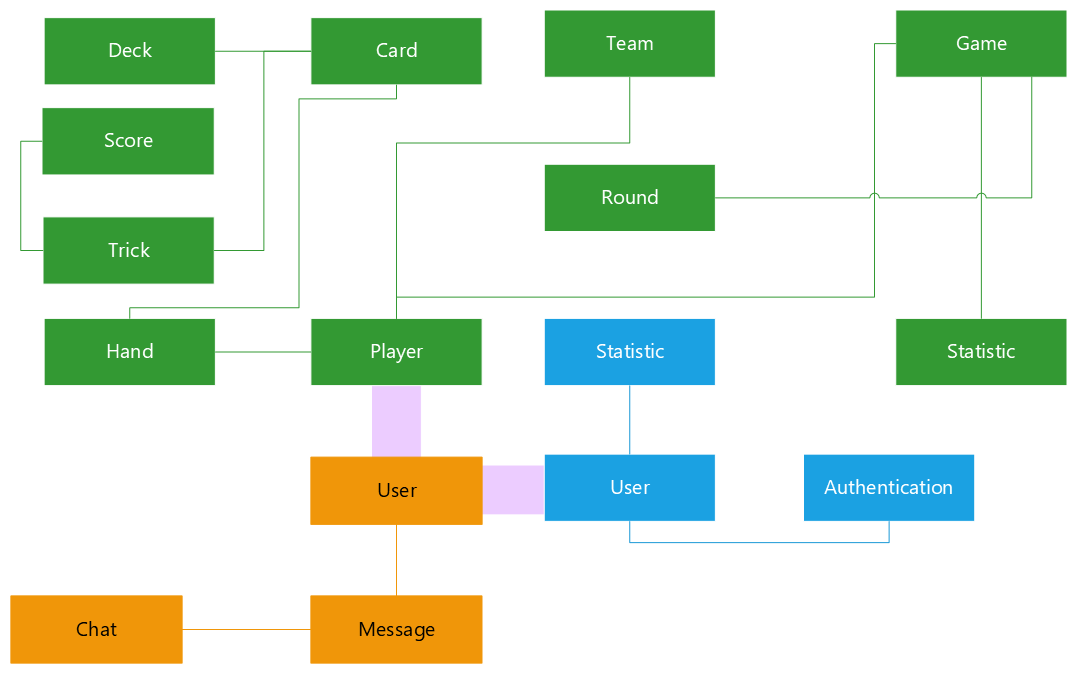
\includegraphics[scale=0.45]{report/img/BoundedCTX.png}
    \caption{Context Map}
    \label{bounded_context}
\end{figure}
\newpage
\section{Requisiti e casi d'uso}
\subsection{Requisiti}
\begin{enumerate}
    \item Account
        \begin{enumerate}
            \item Login
            \item Registrazione
            \item Recupero password
            \item Visualizzazione profilo
            \item Modifica password
            \item Possibilità di scegliere se giocare come ospite o effettuare il login
        \end{enumerate}
    \item Realizzazione partita
        \begin{enumerate}
            \item Creazione partita
            \item Partecipazione partita
            \item gioca carta
            \item Inizio partita
            \item Fine mano
            \item Fine partita
        \end{enumerate}
    \item Chat di gioco
        \begin{enumerate}
            \item chat globale
            \item chat partita
        \end{enumerate}
    \item Possibilità di scegliere un compagno di squadra
    \item Scelta del seme, parole consentite
    \item Modalità di gioco 11 a 0
    \item Gestione punteggio
        \begin{enumerate}
            \item Calcolo totale e parziale (Gestione per ogni mano) del punteggio
            \item Maraffa/Cricca (+3 punti)
        \end{enumerate}
    \item Servizio gestione utenti
    \item Salvataggio statistiche
    \item Realizzazione GUI
        \begin{enumerate}
            \item Refactor della GUI esistente
            \item Rinnovamento GUI
        \end{enumerate}
\end{enumerate}
\subsection{Casi d'uso}
Si riporta di seguito lo schema dei casi d'uso che modella l'interazione dell'utente con l'applicazione.
\begin{figure}[h!]
\centering 
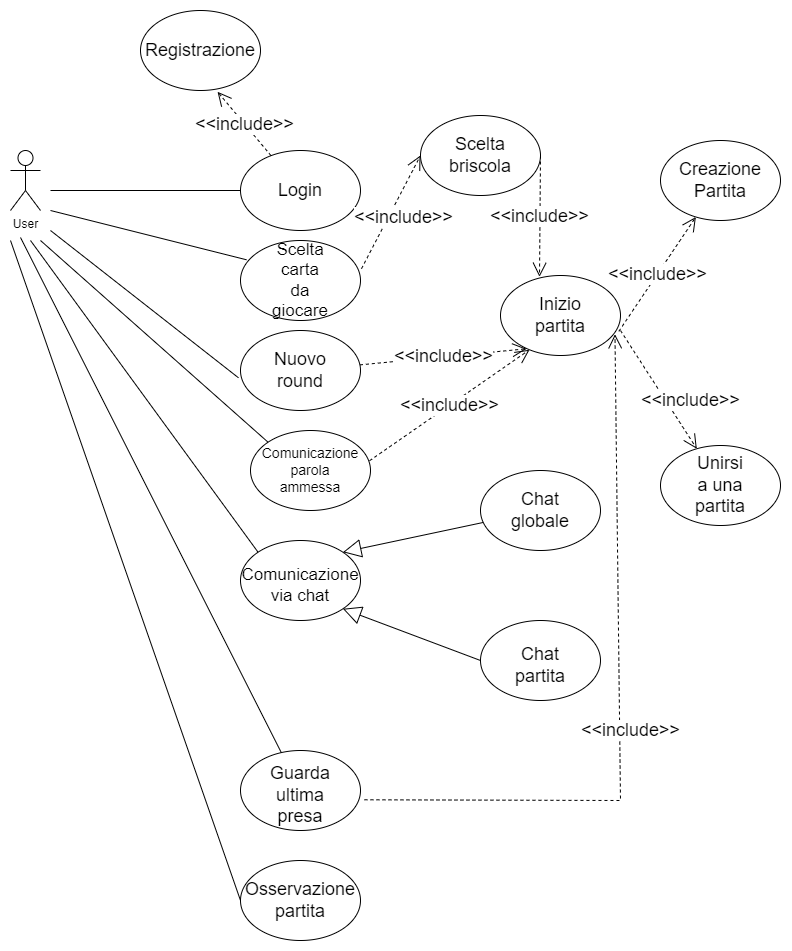
\includegraphics[scale=0.45]{report/img/Casi_duso.png}
\caption{Schema dei casi d'uso}
\label{use_case}
\end{figure}

\section{Design generale del software}

L'architettura del software è basata su micro-servizi autonomi e indipendenti tra loro, la cui comunicazione avviene tramite API REST.
Esiste un middleware che si occupa della gestione e dell'orchestrazione dei micro-servizi, fungendo da ponte per collegare le varie tecnologie.

I microservizi sviluppati si occupano di varie aree legate alla natura del progetto e sono:
\begin{itemize}
    \item \textbf{UserService}: si occupa della gestione degli utenti, quindi la loro registrazione, autenticazione e gestione dei dati personali.
    \item \textbf{BusinessLogic}: si occupa di mantenere al proprio interno tutte le regole del gioco.
    \item \textbf{Front-End}: si occupa di gestire l'interfaccia grafica e la comunicazione con il middleware.
    \item \textbf{Middleware}: si occupa della gestione delle comunicazioni tra i vari microservizi e svolge la funzione di "motore di gioco".
\end{itemize}

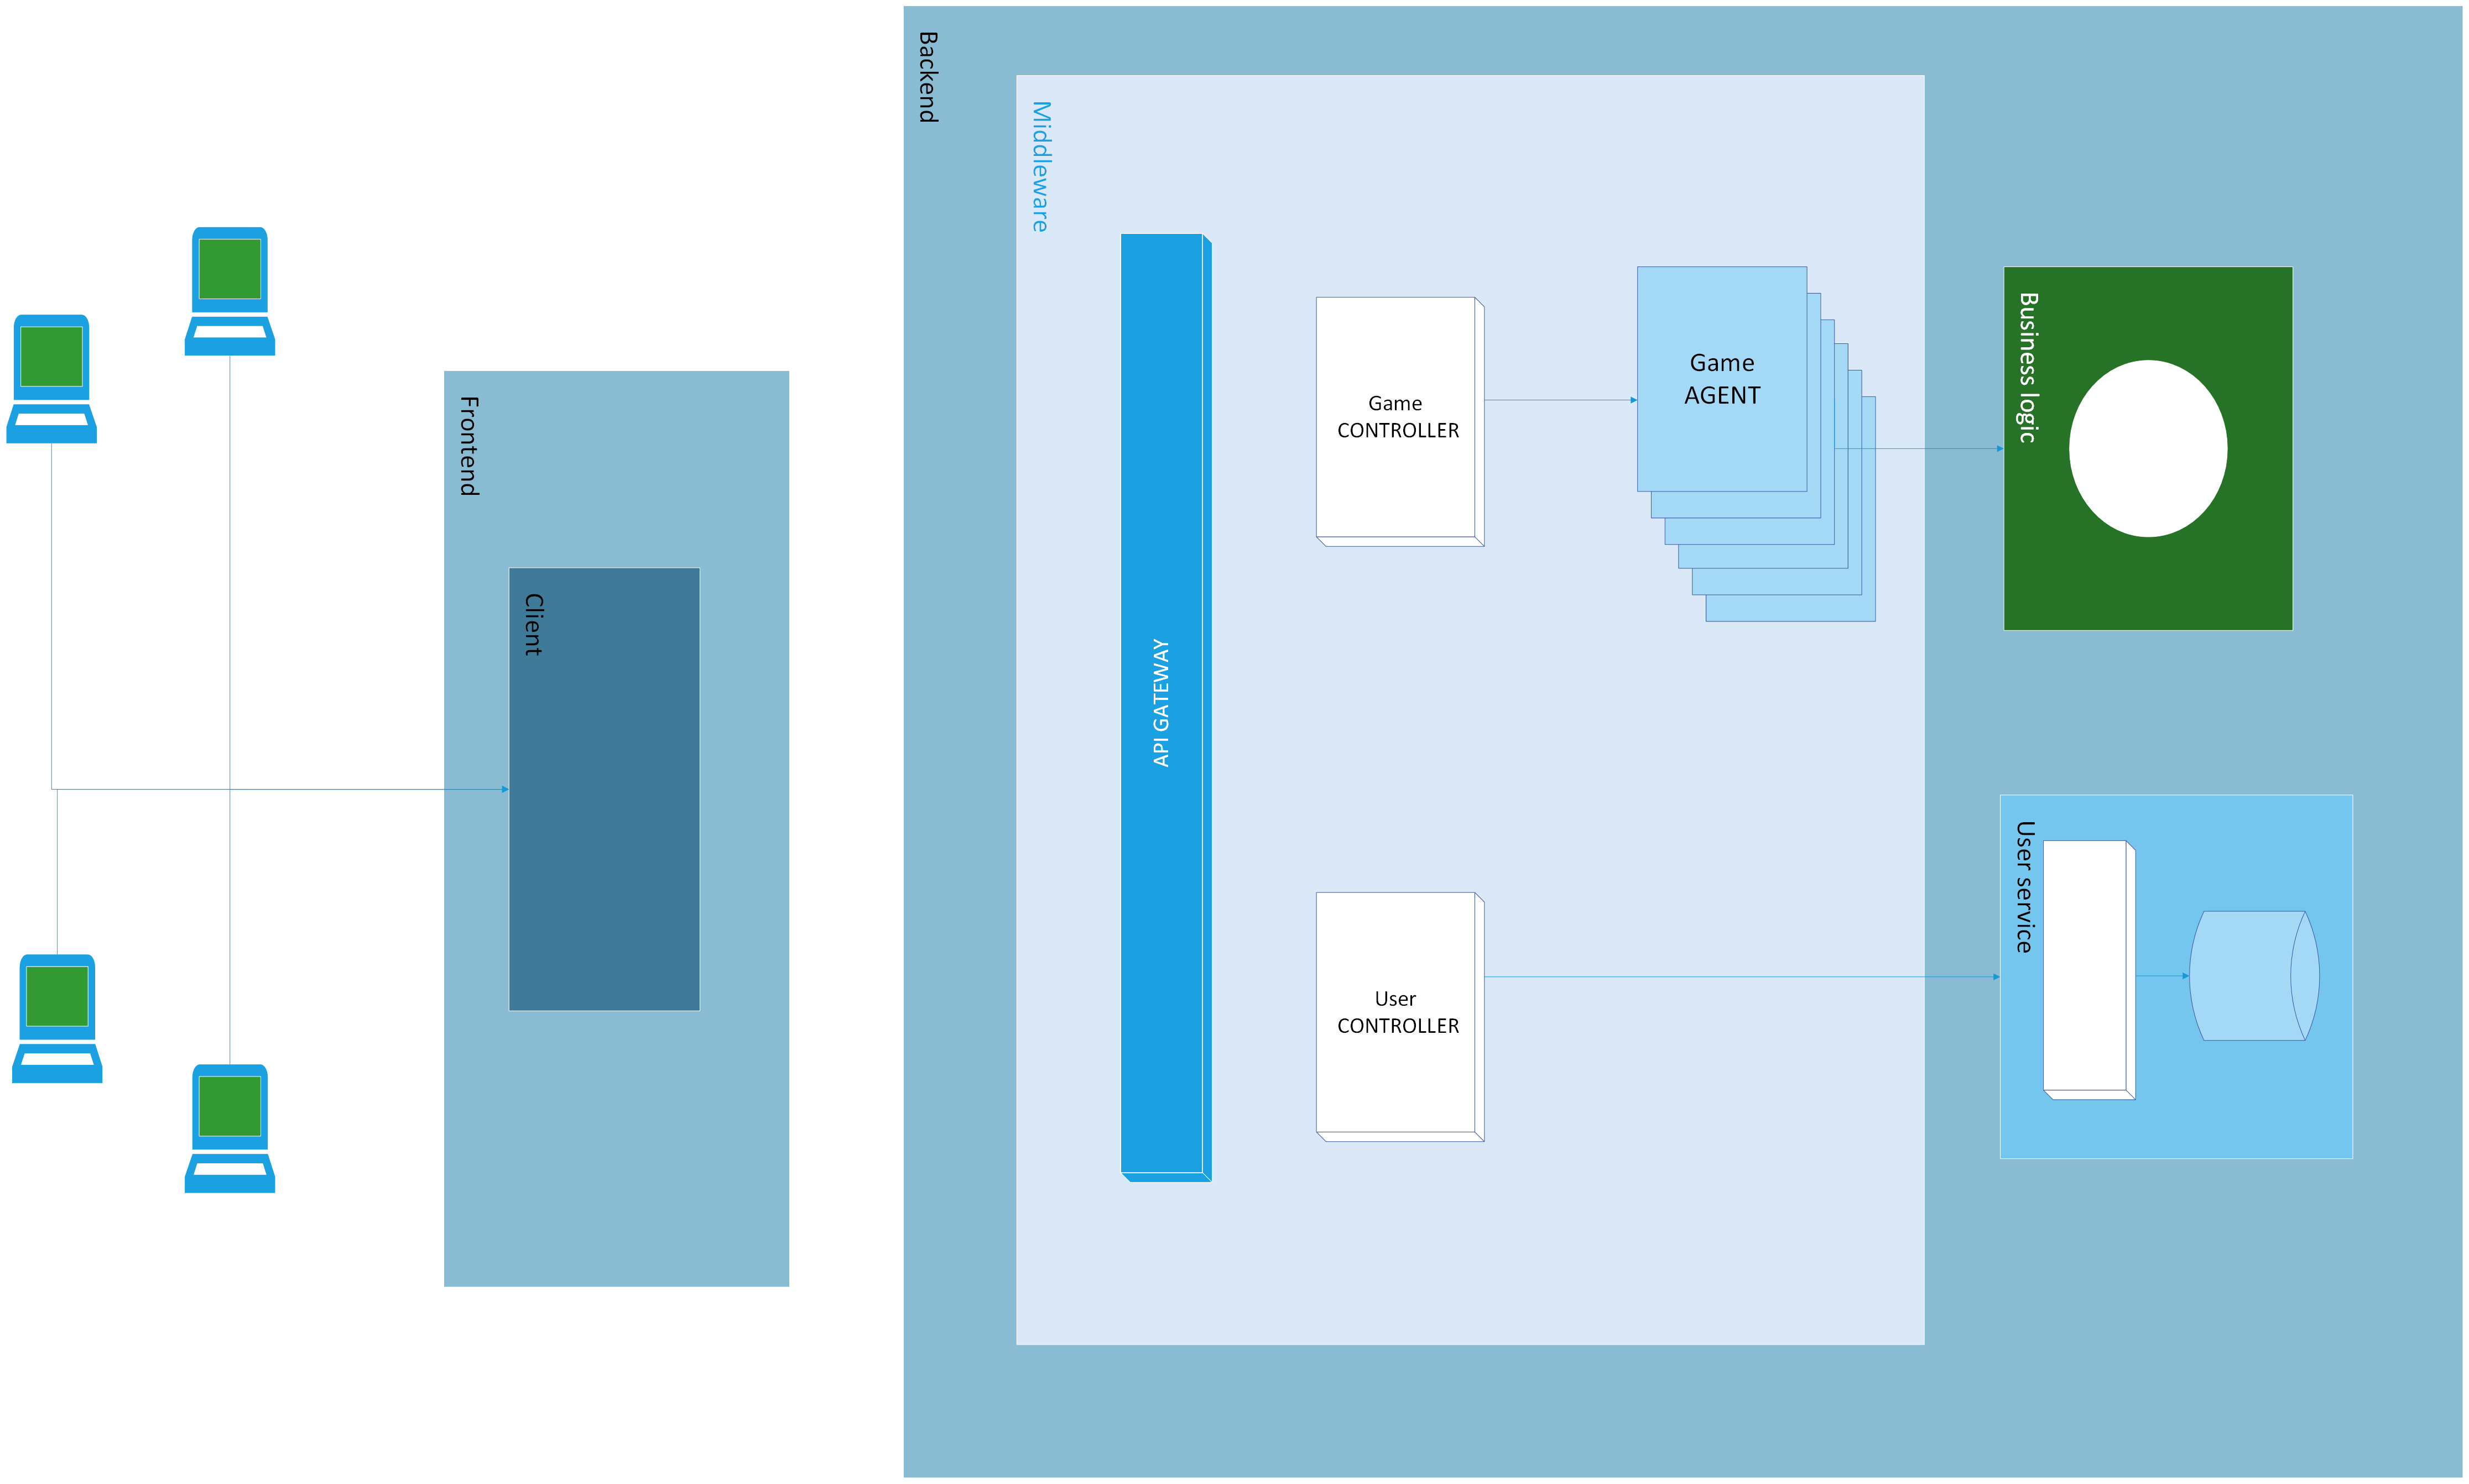
\includegraphics[width=12cm]{report/img/Architecture.png}\\[5.5cm]

\section{Pattern del DDD}

Il pattern di DDD che è stato applicato, data l'architettura del sistema a microservizi, è quello del Consumer-Supplier.
Di seguito, si riportano le motivazione secondo le quali è stato scelto:
\begin{itemize}
    \item servizi loosely coupled
    \item evoluzione indipendente dei servizi, durante l'aggiornamento del sistema.
    \item Ove possibile, ogni bounded context è stato sviluppato in un microservizio separato, ottenendo, così, una distinta separazione della business logic e delle responsabilità. 
    \item chiara definizione del dominio
    \item la \textbf{scalabilità} in base alle richieste del consumer.
    \item La manutenibilità dei singoli componenti che possono, ipoteticamente, essere sviluppati da team diversi in modo parallelo, definendo al meglio i confini del dominio.

\end{itemize}
